\documentclass[twoside]{book}

% Packages required by doxygen
\usepackage{calc}
\usepackage{doxygen}
\usepackage{graphicx}
\usepackage[utf8]{inputenc}
\usepackage{makeidx}
\usepackage{multicol}
\usepackage{multirow}
\usepackage{textcomp}
\usepackage[table]{xcolor}

% NLS support packages
\usepackage[ngerman]{babel}

% Font selection
\usepackage[T1]{fontenc}
\usepackage{mathptmx}
\usepackage[scaled=.90]{helvet}
\usepackage{courier}
\usepackage{amssymb}
\usepackage{sectsty}
\renewcommand{\familydefault}{\sfdefault}
\allsectionsfont{%
  \fontseries{bc}\selectfont%
  \color{darkgray}%
}
\renewcommand{\DoxyLabelFont}{%
  \fontseries{bc}\selectfont%
  \color{darkgray}%
}

% Page & text layout
\usepackage{geometry}
\geometry{%
  a4paper,%
  top=2.5cm,%
  bottom=2.5cm,%
  left=2.5cm,%
  right=2.5cm%
}
\tolerance=750
\hfuzz=15pt
\hbadness=750
\setlength{\emergencystretch}{15pt}
\setlength{\parindent}{0cm}
\setlength{\parskip}{0.2cm}
\makeatletter
\renewcommand{\paragraph}{%
  \@startsection{paragraph}{4}{0ex}{-1.0ex}{1.0ex}{%
    \normalfont\normalsize\bfseries\SS@parafont%
  }%
}
\renewcommand{\subparagraph}{%
  \@startsection{subparagraph}{5}{0ex}{-1.0ex}{1.0ex}{%
    \normalfont\normalsize\bfseries\SS@subparafont%
  }%
}
\makeatother

% Headers & footers
\usepackage{fancyhdr}
\pagestyle{fancyplain}
\fancyhead[LE]{\fancyplain{}{\bfseries\thepage}}
\fancyhead[CE]{\fancyplain{}{}}
\fancyhead[RE]{\fancyplain{}{\bfseries\leftmark}}
\fancyhead[LO]{\fancyplain{}{\bfseries\rightmark}}
\fancyhead[CO]{\fancyplain{}{}}
\fancyhead[RO]{\fancyplain{}{\bfseries\thepage}}
\fancyfoot[LE]{\fancyplain{}{}}
\fancyfoot[CE]{\fancyplain{}{}}
\fancyfoot[RE]{\fancyplain{}{\bfseries\scriptsize Erzeugt am Mit Jun 10 2015 15\-:31\-:49 für Wiesn-\/\-Run von Doxygen }}
\fancyfoot[LO]{\fancyplain{}{\bfseries\scriptsize Erzeugt am Mit Jun 10 2015 15\-:31\-:49 für Wiesn-\/\-Run von Doxygen }}
\fancyfoot[CO]{\fancyplain{}{}}
\fancyfoot[RO]{\fancyplain{}{}}
\renewcommand{\footrulewidth}{0.4pt}
\renewcommand{\chaptermark}[1]{%
  \markboth{#1}{}%
}
\renewcommand{\sectionmark}[1]{%
  \markright{\thesection\ #1}%
}

% Indices & bibliography
\usepackage{natbib}
\usepackage[titles]{tocloft}
\setcounter{tocdepth}{3}
\setcounter{secnumdepth}{5}
\makeindex

% Hyperlinks (required, but should be loaded last)
\usepackage{ifpdf}
\ifpdf
  \usepackage[pdftex,pagebackref=true]{hyperref}
\else
  \usepackage[ps2pdf,pagebackref=true]{hyperref}
\fi
\hypersetup{%
  colorlinks=true,%
  linkcolor=blue,%
  citecolor=blue,%
  unicode%
}

% Custom commands
\newcommand{\clearemptydoublepage}{%
  \newpage{\pagestyle{empty}\cleardoublepage}%
}


%===== C O N T E N T S =====

\begin{document}

% Titlepage & ToC
\hypersetup{pageanchor=false}
\pagenumbering{roman}
\begin{titlepage}
\vspace*{7cm}
\begin{center}%
{\Large Wiesn-\/\-Run }\\
\vspace*{1cm}
{\large Erzeugt von Doxygen 1.8.6}\\
\vspace*{0.5cm}
{\small Mit Jun 10 2015 15:31:49}\\
\end{center}
\end{titlepage}
\clearemptydoublepage
\tableofcontents
\clearemptydoublepage
\pagenumbering{arabic}
\hypersetup{pageanchor=true}

%--- Begin generated contents ---
\chapter{Ausstehende Aufgaben}
\label{todo}
\hypertarget{todo}{}

\begin{DoxyRefList}
\item[\label{todo__todo000001}%
\hypertarget{todo__todo000001}{}%
Klasse \hyperlink{structscoreStruct}{score\-Struct} ]Das Konzept der Alkohol-\/\-Punkte muss noch ausgearbeitet werden. \begin{DoxyAuthor}{Autor}
Simon  
\end{DoxyAuthor}

\item[\label{todo__todo000002}%
\hypertarget{todo__todo000002}{}%
Klasse \hyperlink{structstateStruct}{state\-Struct} ]Es fehlen noch die States selbst. \begin{DoxyAuthor}{Autor}
Simon 
\end{DoxyAuthor}

\end{DoxyRefList}
\chapter{Hierarchie-\/\-Verzeichnis}
\section{Klassenhierarchie}
Die Liste der Ableitungen ist -\/mit Einschränkungen-\/ alphabetisch sortiert\-:\begin{DoxyCompactList}
\item \contentsline{section}{Audio}{\pageref{classAudio}}{}
\item \contentsline{section}{Audio\-Control}{\pageref{classAudioControl}}{}
\item \contentsline{section}{event\-Struct}{\pageref{structeventStruct}}{}
\item \contentsline{section}{Game}{\pageref{classGame}}{}
\item \contentsline{section}{Game\-Object}{\pageref{classGameObject}}{}
\begin{DoxyCompactList}
\item \contentsline{section}{Moving\-Object}{\pageref{classMovingObject}}{}
\begin{DoxyCompactList}
\item \contentsline{section}{Enemy}{\pageref{classEnemy}}{}
\item \contentsline{section}{Player}{\pageref{classPlayer}}{}
\item \contentsline{section}{Shoot}{\pageref{classShoot}}{}
\end{DoxyCompactList}
\end{DoxyCompactList}
\item \contentsline{section}{Input}{\pageref{classInput}}{}
\item \contentsline{section}{Render\-Attack}{\pageref{classRenderAttack}}{}
\item \contentsline{section}{Render\-Background}{\pageref{classRenderBackground}}{}
\item \contentsline{section}{Render\-Enemy}{\pageref{classRenderEnemy}}{}
\item \contentsline{section}{Render\-Gui\-Element}{\pageref{classRenderGuiElement}}{}
\item \contentsline{section}{Render\-Obstacle}{\pageref{classRenderObstacle}}{}
\item \contentsline{section}{Render\-Player}{\pageref{classRenderPlayer}}{}
\item \contentsline{section}{score\-Struct}{\pageref{structscoreStruct}}{}
\item \contentsline{section}{state\-Struct}{\pageref{structstateStruct}}{}
\end{DoxyCompactList}

\chapter{Klassen-\/\-Verzeichnis}
\section{Auflistung der Klassen}
Hier folgt die Aufzählung aller Klassen, Strukturen, Varianten und Schnittstellen mit einer Kurzbeschreibung\-:\begin{DoxyCompactList}
\item\contentsline{section}{\hyperlink{classAudio}{Audio} }{\pageref{classAudio}}{}
\item\contentsline{section}{\hyperlink{classAudioControl}{Audio\-Control} }{\pageref{classAudioControl}}{}
\item\contentsline{section}{\hyperlink{classEnemy}{Enemy} }{\pageref{classEnemy}}{}
\item\contentsline{section}{\hyperlink{structeventStruct}{event\-Struct} \\*Struktur für die Events Enthält object\-A als Objekt, aus dessen Sicht die Kollision berechnet wurde. object\-A ist immer ein \hyperlink{classMovingObject}{Moving\-Object}, object\-B kann beides sein. Die Art und Richtung der Kollision werden mit gespeichert }{\pageref{structeventStruct}}{}
\item\contentsline{section}{\hyperlink{classGame}{Game} }{\pageref{classGame}}{}
\item\contentsline{section}{\hyperlink{classGameObject}{Game\-Object} }{\pageref{classGameObject}}{}
\item\contentsline{section}{\hyperlink{classInput}{Input} }{\pageref{classInput}}{}
\item\contentsline{section}{\hyperlink{classMovingObject}{Moving\-Object} }{\pageref{classMovingObject}}{}
\item\contentsline{section}{\hyperlink{classPlayer}{Player} }{\pageref{classPlayer}}{}
\item\contentsline{section}{\hyperlink{classRenderAttack}{Render\-Attack} }{\pageref{classRenderAttack}}{}
\item\contentsline{section}{\hyperlink{classRenderBackground}{Render\-Background} }{\pageref{classRenderBackground}}{}
\item\contentsline{section}{\hyperlink{classRenderEnemy}{Render\-Enemy} }{\pageref{classRenderEnemy}}{}
\item\contentsline{section}{\hyperlink{classRenderGuiElement}{Render\-Gui\-Element} }{\pageref{classRenderGuiElement}}{}
\item\contentsline{section}{\hyperlink{classRenderObstacle}{Render\-Obstacle} }{\pageref{classRenderObstacle}}{}
\item\contentsline{section}{\hyperlink{classRenderPlayer}{Render\-Player} }{\pageref{classRenderPlayer}}{}
\item\contentsline{section}{\hyperlink{structscoreStruct}{score\-Struct} \\*Struktur für die Score des Spielers In dieser Struktur werden getötete Gegner, zurückgelegte Entfernung und Alkohol-\/\-Punkte gespeichert. Alkohol-\/\-Punkte erhält der Spieler für einen gewissen Pegel in einem Zeitabschnitt }{\pageref{structscoreStruct}}{}
\item\contentsline{section}{\hyperlink{classShoot}{Shoot} }{\pageref{classShoot}}{}
\item\contentsline{section}{\hyperlink{structstateStruct}{state\-Struct} \\*Struktur für die States des Spiels Sowohl Sound-\/ als auch Grafik-\/\-Ausgabe erhalten aus den States Informationen darüber, was gerade im Spiel passiert, z.\-B. dass gerade der Spieler angreift, ein Gegner stribt etc }{\pageref{structstateStruct}}{}
\end{DoxyCompactList}

\chapter{Klassen-\/\-Dokumentation}
\hypertarget{classAudio}{\section{Audio Klassenreferenz}
\label{classAudio}\index{Audio@{Audio}}
}


Die Dokumentation für diese Klasse wurde erzeugt aufgrund der Dateien\-:\begin{DoxyCompactItemize}
\item 
Wiesn-\/\-Run/src/audio.\-h\item 
Wiesn-\/\-Run/src/audio.\-cpp\end{DoxyCompactItemize}

\hypertarget{classAudioControl}{\section{Audio\-Control Klassenreferenz}
\label{classAudioControl}\index{Audio\-Control@{Audio\-Control}}
}


Die Dokumentation für diese Klasse wurde erzeugt aufgrund der Dateien\-:\begin{DoxyCompactItemize}
\item 
Wiesn-\/\-Run/src/audiocontrol.\-h\item 
Wiesn-\/\-Run/src/audiocontrol.\-cpp\end{DoxyCompactItemize}

\hypertarget{classEnemy}{\section{Enemy Klassenreferenz}
\label{classEnemy}\index{Enemy@{Enemy}}
}
Klassendiagramm für Enemy\-:\begin{figure}[H]
\begin{center}
\leavevmode
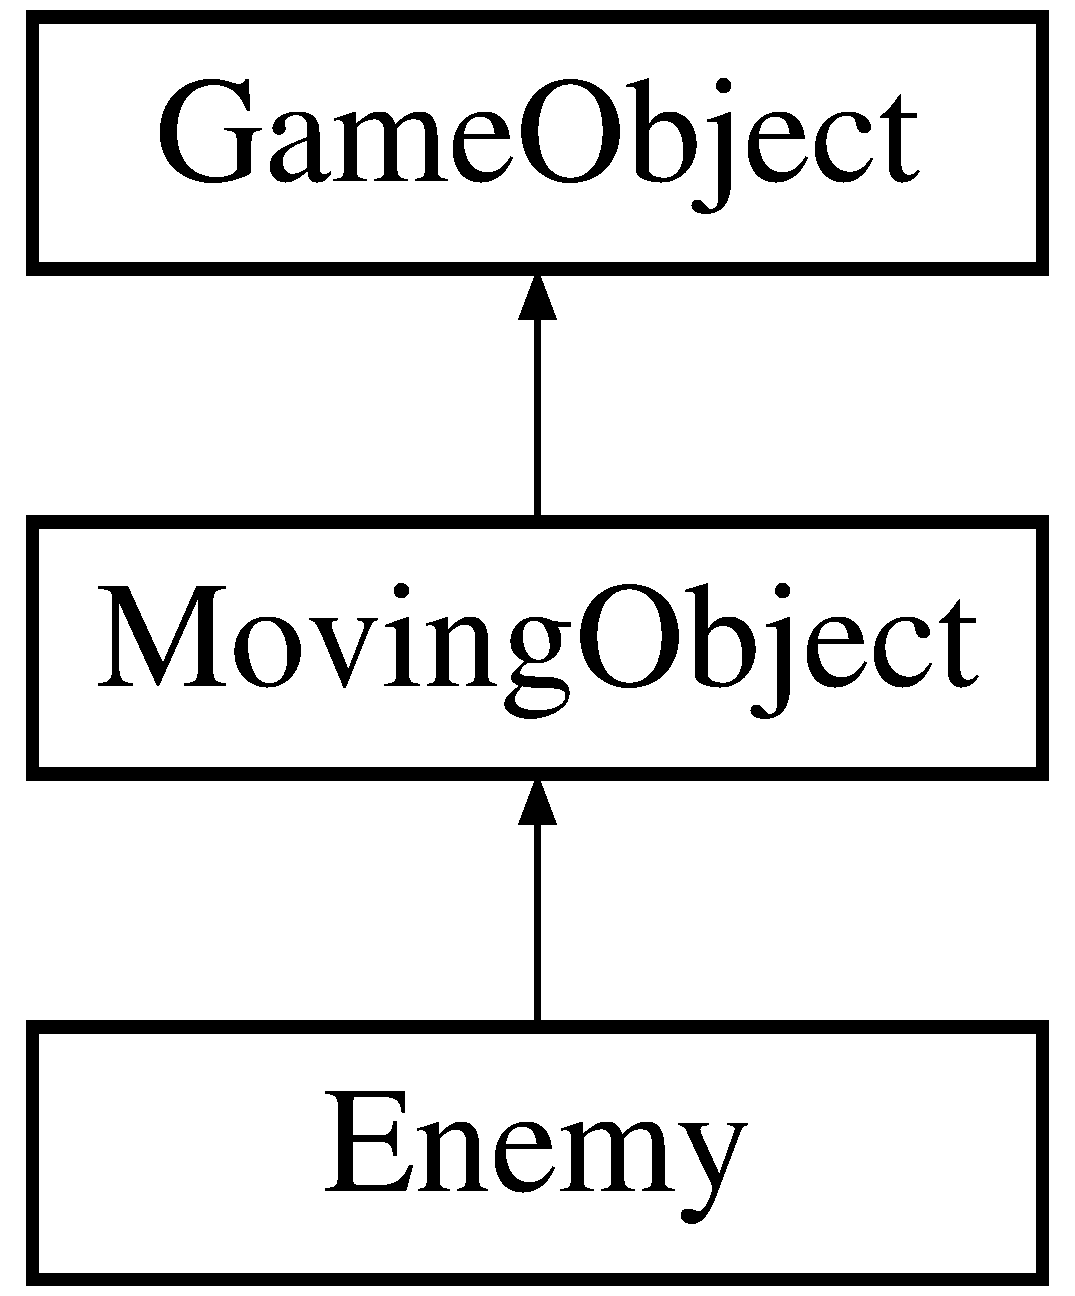
\includegraphics[height=3.000000cm]{classEnemy}
\end{center}
\end{figure}
\subsection*{Öffentliche Methoden}
\begin{DoxyCompactItemize}
\item 
\hypertarget{classEnemy_ae9cfe69594b5fabec06d22f77ddce202}{int {\bfseries get\-Health} () const }\label{classEnemy_ae9cfe69594b5fabec06d22f77ddce202}

\item 
\hypertarget{classEnemy_a48f9331e93449f27c8d6374c75c81363}{void {\bfseries set\-Health} (int health)}\label{classEnemy_a48f9331e93449f27c8d6374c75c81363}

\item 
\hypertarget{classEnemy_a5f969adca5809e5ff5a83ef20b19826d}{int {\bfseries get\-Inflicted\-Damage} () const }\label{classEnemy_a5f969adca5809e5ff5a83ef20b19826d}

\item 
\hypertarget{classEnemy_aae82e3d3056d5981037100683bdae94d}{bool {\bfseries get\-Death} () const }\label{classEnemy_aae82e3d3056d5981037100683bdae94d}

\item 
\hypertarget{classEnemy_a749a1a8932d9b067e3770fb1425f216b}{void {\bfseries set\-Death} (bool death)}\label{classEnemy_a749a1a8932d9b067e3770fb1425f216b}

\item 
\hypertarget{classEnemy_ad55ee71b5a8c23fbd00b3c368b90cc64}{void {\bfseries update} ()}\label{classEnemy_ad55ee71b5a8c23fbd00b3c368b90cc64}

\end{DoxyCompactItemize}
\subsection*{Weitere Geerbte Elemente}


Die Dokumentation für diese Klasse wurde erzeugt aufgrund der Dateien\-:\begin{DoxyCompactItemize}
\item 
Wiesn-\/\-Run/src/enemy.\-h\item 
Wiesn-\/\-Run/src/enemy.\-cpp\end{DoxyCompactItemize}

\hypertarget{structeventStruct}{\section{event\-Struct Strukturreferenz}
\label{structeventStruct}\index{event\-Struct@{event\-Struct}}
}


Struktur für die Events Enthält object\-A als Objekt, aus dessen Sicht die Kollision berechnet wurde. object\-A ist immer ein \hyperlink{classMovingObject}{Moving\-Object}, object\-B kann beides sein. Die Art und Richtung der Kollision werden mit gespeichert.  




{\ttfamily \#include $<$definitions.\-h$>$}

\subsection*{Öffentliche Attribute}
\begin{DoxyCompactItemize}
\item 
\hypertarget{structeventStruct_aa8c0da4707f8c8a8c750e07c97d4de22}{\hyperlink{classGameObject}{Game\-Object} {\bfseries object\-A}}\label{structeventStruct_aa8c0da4707f8c8a8c750e07c97d4de22}

\item 
\hypertarget{structeventStruct_af30f5189c083e03fb4b55477f30df7db}{\hyperlink{classGameObject}{Game\-Object} {\bfseries object\-B}}\label{structeventStruct_af30f5189c083e03fb4b55477f30df7db}

\item 
\hypertarget{structeventStruct_a4fc24ec95611cc3aebca2e2f84fb3551}{enum collision\-Type {\bfseries collision}}\label{structeventStruct_a4fc24ec95611cc3aebca2e2f84fb3551}

\item 
\hypertarget{structeventStruct_ada2513a58c2804a3d18345f895e43815}{enum collision\-Direction {\bfseries direction}}\label{structeventStruct_ada2513a58c2804a3d18345f895e43815}

\end{DoxyCompactItemize}


\subsection{Ausführliche Beschreibung}
Struktur für die Events Enthält object\-A als Objekt, aus dessen Sicht die Kollision berechnet wurde. object\-A ist immer ein \hyperlink{classMovingObject}{Moving\-Object}, object\-B kann beides sein. Die Art und Richtung der Kollision werden mit gespeichert. 

\begin{DoxyAuthor}{Autor}
Simon 
\end{DoxyAuthor}


Die Dokumentation für diese Struktur wurde erzeugt aufgrund der Datei\-:\begin{DoxyCompactItemize}
\item 
Wiesn-\/\-Run/src/definitions.\-h\end{DoxyCompactItemize}

\hypertarget{classGame}{\section{Game Klassenreferenz}
\label{classGame}\index{Game@{Game}}
}
\subsection*{Öffentliche Methoden}
\begin{DoxyCompactItemize}
\item 
\hypertarget{classGame_ae8638ccdb0ef3bf39a6affa30aa1258f}{void \hyperlink{classGame_ae8638ccdb0ef3bf39a6affa30aa1258f}{start\-Game} ()}\label{classGame_ae8638ccdb0ef3bf39a6affa30aa1258f}

\begin{DoxyCompactList}\small\item\em Startet das Spiel, wird einmalig von main() aufgerufen. \end{DoxyCompactList}\end{DoxyCompactItemize}
\subsection*{Öffentliche Attribute}
\begin{DoxyCompactItemize}
\item 
\hypertarget{classGame_a14bc24b16362834be072dca921c8c154}{std\-::list$<$ struct \hyperlink{structeventStruct}{event\-Struct} $>$ {\bfseries events\-To\-Handle}}\label{classGame_a14bc24b16362834be072dca921c8c154}

\end{DoxyCompactItemize}


Die Dokumentation für diese Klasse wurde erzeugt aufgrund der Dateien\-:\begin{DoxyCompactItemize}
\item 
Wiesn-\/\-Run/src/game.\-h\item 
Wiesn-\/\-Run/src/game.\-cpp\end{DoxyCompactItemize}

\hypertarget{classGameObject}{\section{Game\-Object Klassenreferenz}
\label{classGameObject}\index{Game\-Object@{Game\-Object}}
}
Klassendiagramm für Game\-Object\-:\begin{figure}[H]
\begin{center}
\leavevmode
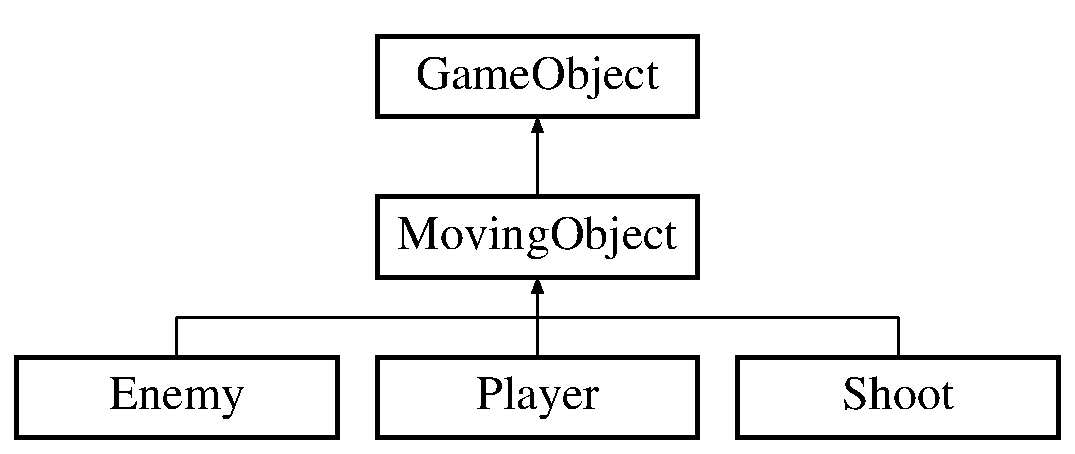
\includegraphics[height=3.000000cm]{classGameObject}
\end{center}
\end{figure}
\subsection*{Öffentliche Methoden}
\begin{DoxyCompactItemize}
\item 
\hypertarget{classGameObject_ab927cea08154292d6f4ab73c3fb9351b}{{\bfseries Game\-Object} (int pos\-X, int pos\-Y, int length, int height, consistency\-Type collusion\-Type, object\-Type type)}\label{classGameObject_ab927cea08154292d6f4ab73c3fb9351b}

\item 
\hypertarget{classGameObject_a92433f7589ed0c8053e06bd468d81be6}{int {\bfseries get\-Pos\-X} () const }\label{classGameObject_a92433f7589ed0c8053e06bd468d81be6}

\item 
\hypertarget{classGameObject_a30cd47267461d569b2b601edb2c849c8}{int {\bfseries get\-Pos\-Y} () const }\label{classGameObject_a30cd47267461d569b2b601edb2c849c8}

\item 
\hypertarget{classGameObject_a172ffc6cb61b0da947f3eabbba57ef51}{int {\bfseries get\-Length} () const }\label{classGameObject_a172ffc6cb61b0da947f3eabbba57ef51}

\item 
\hypertarget{classGameObject_a2553f445dc1aa30defaa3bc0875927ba}{int {\bfseries get\-Height} () const }\label{classGameObject_a2553f445dc1aa30defaa3bc0875927ba}

\item 
\hypertarget{classGameObject_ad13359758249110f2a895902b5bd290f}{object\-Type {\bfseries get\-Type} () const }\label{classGameObject_ad13359758249110f2a895902b5bd290f}

\item 
\hypertarget{classGameObject_abb24a9a876a528285b394753c8a38c42}{collision\-Type {\bfseries get\-Collision\-Type} () const }\label{classGameObject_abb24a9a876a528285b394753c8a38c42}

\end{DoxyCompactItemize}
\subsection*{Geschützte Attribute}
\begin{DoxyCompactItemize}
\item 
\hypertarget{classGameObject_a02b13dc4d29636ea6e7c66ac90e5198f}{int {\bfseries pos\-X}}\label{classGameObject_a02b13dc4d29636ea6e7c66ac90e5198f}

\item 
\hypertarget{classGameObject_a8bce50c4f2732c4ceff89aac8525efa2}{int {\bfseries pos\-Y}}\label{classGameObject_a8bce50c4f2732c4ceff89aac8525efa2}

\item 
\hypertarget{classGameObject_a1e34c9fc69dc662a5193907727222666}{consistency\-Type {\bfseries collision\-Type}}\label{classGameObject_a1e34c9fc69dc662a5193907727222666}

\end{DoxyCompactItemize}


Die Dokumentation für diese Klasse wurde erzeugt aufgrund der Dateien\-:\begin{DoxyCompactItemize}
\item 
Wiesn-\/\-Run/src/gameobject.\-h\item 
Wiesn-\/\-Run/src/gameobject.\-cpp\end{DoxyCompactItemize}

\hypertarget{classInput}{\section{Input Klassenreferenz}
\label{classInput}\index{Input@{Input}}
}


Die Dokumentation für diese Klasse wurde erzeugt aufgrund der Dateien\-:\begin{DoxyCompactItemize}
\item 
Wiesn-\/\-Run/src/input.\-h\item 
Wiesn-\/\-Run/src/input.\-cpp\end{DoxyCompactItemize}

\hypertarget{classMovingObject}{\section{Moving\-Object Klassenreferenz}
\label{classMovingObject}\index{Moving\-Object@{Moving\-Object}}
}
Klassendiagramm für Moving\-Object\-:\begin{figure}[H]
\begin{center}
\leavevmode
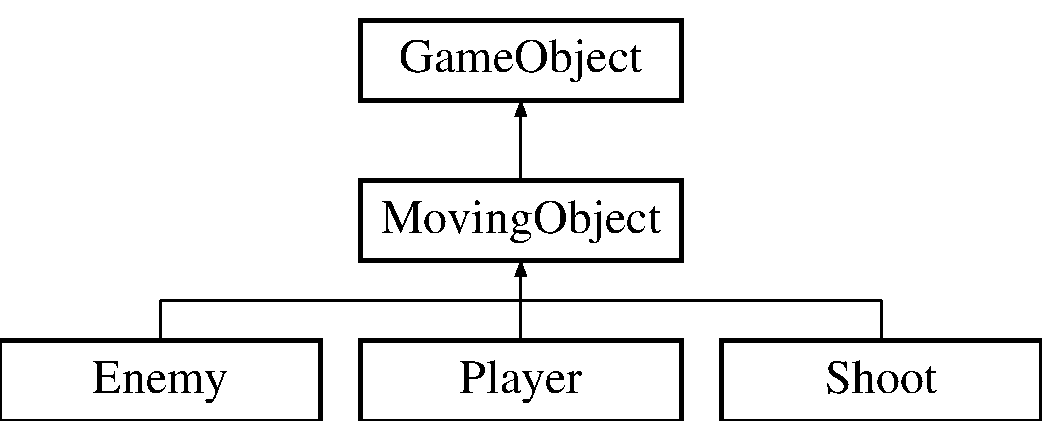
\includegraphics[height=3.000000cm]{classMovingObject}
\end{center}
\end{figure}
\subsection*{Öffentliche Methoden}
\begin{DoxyCompactItemize}
\item 
\hypertarget{classMovingObject_ab0abd688a3a564fde58c1753975ecaf1}{void {\bfseries set\-Pos\-X} (int pos\-X)}\label{classMovingObject_ab0abd688a3a564fde58c1753975ecaf1}

\item 
\hypertarget{classMovingObject_ad2e1227ea79fbc5ea1d6903b3f5140b3}{void {\bfseries set\-Pos\-Y} (int pos\-Y)}\label{classMovingObject_ad2e1227ea79fbc5ea1d6903b3f5140b3}

\item 
\hypertarget{classMovingObject_ac79f660b3543f5afb84205b8715c3282}{int {\bfseries get\-Speed\-X} () const }\label{classMovingObject_ac79f660b3543f5afb84205b8715c3282}

\item 
\hypertarget{classMovingObject_a8ed63e698a611f8a778747719cc63a24}{int {\bfseries get\-Speed\-Y} () const }\label{classMovingObject_a8ed63e698a611f8a778747719cc63a24}

\item 
\hypertarget{classMovingObject_af6721c8115b2cb97b119759a0fb8f60b}{void {\bfseries set\-Speed\-X} (int speed\-X)}\label{classMovingObject_af6721c8115b2cb97b119759a0fb8f60b}

\item 
\hypertarget{classMovingObject_a98dce0d944435d37c7f06f655afa9fea}{void {\bfseries set\-Speed\-Y} (int speed\-Y)}\label{classMovingObject_a98dce0d944435d37c7f06f655afa9fea}

\item 
\hypertarget{classMovingObject_a8614d585f9c38901ad41dd5d35384e1e}{virtual void {\bfseries update} ()}\label{classMovingObject_a8614d585f9c38901ad41dd5d35384e1e}

\end{DoxyCompactItemize}
\subsection*{Geschützte Methoden}
\begin{DoxyCompactItemize}
\item 
\hypertarget{classMovingObject_ad3305f90847ca544c780c91ac5351fc0}{void {\bfseries update\-Position} ()}\label{classMovingObject_ad3305f90847ca544c780c91ac5351fc0}

\end{DoxyCompactItemize}
\subsection*{Weitere Geerbte Elemente}


Die Dokumentation für diese Klasse wurde erzeugt aufgrund der Dateien\-:\begin{DoxyCompactItemize}
\item 
Wiesn-\/\-Run/src/movingobject.\-h\item 
Wiesn-\/\-Run/src/movingobject.\-cpp\end{DoxyCompactItemize}

\hypertarget{classPlayer}{\section{Player Klassenreferenz}
\label{classPlayer}\index{Player@{Player}}
}
Klassendiagramm für Player\-:\begin{figure}[H]
\begin{center}
\leavevmode
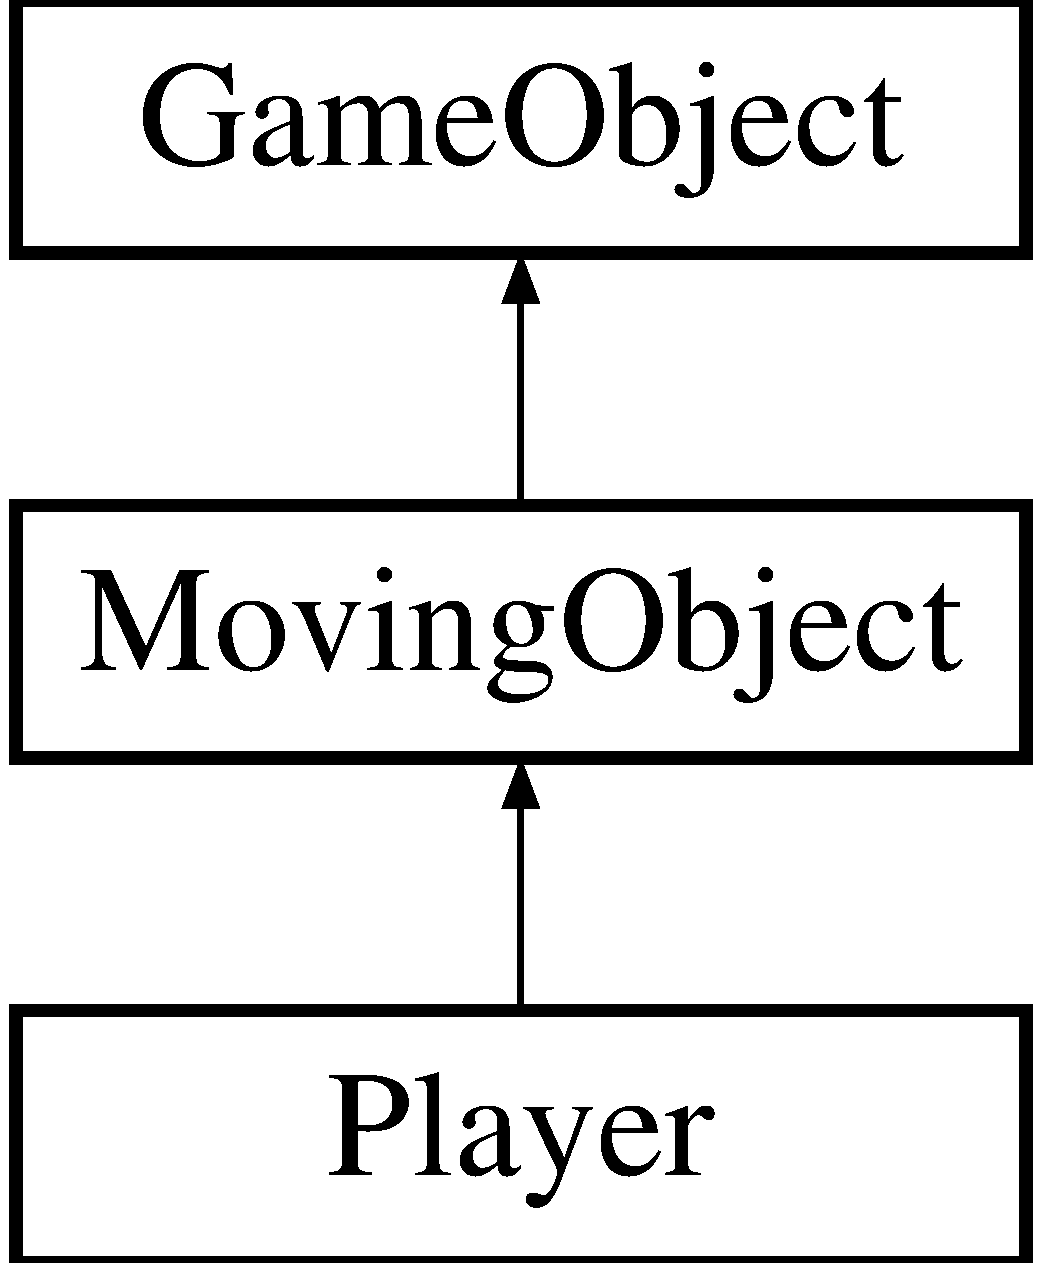
\includegraphics[height=3.000000cm]{classPlayer}
\end{center}
\end{figure}
\subsection*{Öffentliche Methoden}
\begin{DoxyCompactItemize}
\item 
\hypertarget{classPlayer_a3042adb49808b2629137f4d85b6b5fd3}{int {\bfseries get\-Health} () const }\label{classPlayer_a3042adb49808b2629137f4d85b6b5fd3}

\item 
\hypertarget{classPlayer_a8f28f6b069f7388877e02ae0a175d4ab}{void {\bfseries set\-Health} (int health)}\label{classPlayer_a8f28f6b069f7388877e02ae0a175d4ab}

\item 
\hypertarget{classPlayer_a486b82d4d244039a03d387d41885650b}{int {\bfseries get\-Alcohol\-Level} () const }\label{classPlayer_a486b82d4d244039a03d387d41885650b}

\item 
\hypertarget{classPlayer_a59ca71be81f1f60884c183bcb59ec180}{void {\bfseries increase\-Alcohol\-Level} (int additional\-Alcohol)}\label{classPlayer_a59ca71be81f1f60884c183bcb59ec180}

\item 
\hypertarget{classPlayer_a169348f8fee6e5fcd226666c5d0828bf}{void {\bfseries decrease\-Alcohol\-Level} ()}\label{classPlayer_a169348f8fee6e5fcd226666c5d0828bf}

\item 
\hypertarget{classPlayer_af1f0af69e333caf0433f760a3eec6278}{int {\bfseries get\-Ammunatiuon} () const }\label{classPlayer_af1f0af69e333caf0433f760a3eec6278}

\item 
\hypertarget{classPlayer_a7e55451588b8cada842cdb255066e434}{void {\bfseries increase\-Ammunation} ()}\label{classPlayer_a7e55451588b8cada842cdb255066e434}

\item 
\hypertarget{classPlayer_a2f0f8c03a11e3f41d1ca511533b67b9b}{void {\bfseries decrease\-Ammunation} ()}\label{classPlayer_a2f0f8c03a11e3f41d1ca511533b67b9b}

\item 
\hypertarget{classPlayer_a99a3c0636d141ffeecfe3c83e772b787}{int {\bfseries get\-Immunity\-Cooldown} () const }\label{classPlayer_a99a3c0636d141ffeecfe3c83e772b787}

\item 
\hypertarget{classPlayer_a360fe426d92da74fdbff2bffec48b863}{void {\bfseries set\-Immunity\-Cooldown} (int immunity\-Cooldown)}\label{classPlayer_a360fe426d92da74fdbff2bffec48b863}

\item 
\hypertarget{classPlayer_a592d25e24da471c9d92d90e5019a581b}{void {\bfseries set\-Jump} (bool jump)}\label{classPlayer_a592d25e24da471c9d92d90e5019a581b}

\item 
\hypertarget{classPlayer_a35738295086ff15f3317a2ce46a25f30}{void {\bfseries set\-Fall} ()}\label{classPlayer_a35738295086ff15f3317a2ce46a25f30}

\item 
\hypertarget{classPlayer_a9f859b8531d3af6262e6f925b8702cc8}{void {\bfseries reset\-Jump} ()}\label{classPlayer_a9f859b8531d3af6262e6f925b8702cc8}

\item 
\hypertarget{classPlayer_a82c3476f3e65a4e2ac6bcd040771bdd4}{void {\bfseries update} ()}\label{classPlayer_a82c3476f3e65a4e2ac6bcd040771bdd4}

\end{DoxyCompactItemize}
\subsection*{Weitere Geerbte Elemente}


Die Dokumentation für diese Klasse wurde erzeugt aufgrund der Dateien\-:\begin{DoxyCompactItemize}
\item 
Wiesn-\/\-Run/src/player.\-h\item 
Wiesn-\/\-Run/src/player.\-cpp\end{DoxyCompactItemize}

\hypertarget{classRenderAttack}{\section{Render\-Attack Klassenreferenz}
\label{classRenderAttack}\index{Render\-Attack@{Render\-Attack}}
}


Die Dokumentation für diese Klasse wurde erzeugt aufgrund der Dateien\-:\begin{DoxyCompactItemize}
\item 
Wiesn-\/\-Run/src/renderattack.\-h\item 
Wiesn-\/\-Run/src/renderattack.\-cpp\end{DoxyCompactItemize}

\hypertarget{classRenderBackground}{\section{Render\-Background Klassenreferenz}
\label{classRenderBackground}\index{Render\-Background@{Render\-Background}}
}


Die Dokumentation für diese Klasse wurde erzeugt aufgrund der Dateien\-:\begin{DoxyCompactItemize}
\item 
Wiesn-\/\-Run/src/renderbackground.\-h\item 
Wiesn-\/\-Run/src/renderbackground.\-cpp\end{DoxyCompactItemize}

\hypertarget{classRenderEnemy}{\section{Render\-Enemy Klassenreferenz}
\label{classRenderEnemy}\index{Render\-Enemy@{Render\-Enemy}}
}


Die Dokumentation für diese Klasse wurde erzeugt aufgrund der Dateien\-:\begin{DoxyCompactItemize}
\item 
Wiesn-\/\-Run/src/renderenemy.\-h\item 
Wiesn-\/\-Run/src/renderenemy.\-cpp\end{DoxyCompactItemize}

\hypertarget{classRenderGuiElement}{\section{Render\-Gui\-Element Klassenreferenz}
\label{classRenderGuiElement}\index{Render\-Gui\-Element@{Render\-Gui\-Element}}
}


Die Dokumentation für diese Klasse wurde erzeugt aufgrund der Dateien\-:\begin{DoxyCompactItemize}
\item 
Wiesn-\/\-Run/src/renderguielement.\-h\item 
Wiesn-\/\-Run/src/renderguielement.\-cpp\end{DoxyCompactItemize}

\hypertarget{classRenderObstacle}{\section{Render\-Obstacle Klassenreferenz}
\label{classRenderObstacle}\index{Render\-Obstacle@{Render\-Obstacle}}
}


Die Dokumentation für diese Klasse wurde erzeugt aufgrund der Dateien\-:\begin{DoxyCompactItemize}
\item 
Wiesn-\/\-Run/src/renderobstacle.\-h\item 
Wiesn-\/\-Run/src/renderobstacle.\-cpp\end{DoxyCompactItemize}

\hypertarget{classRenderPlayer}{\section{Render\-Player Klassenreferenz}
\label{classRenderPlayer}\index{Render\-Player@{Render\-Player}}
}


Die Dokumentation für diese Klasse wurde erzeugt aufgrund der Dateien\-:\begin{DoxyCompactItemize}
\item 
Wiesn-\/\-Run/src/renderplayer.\-h\item 
Wiesn-\/\-Run/src/renderplayer.\-cpp\end{DoxyCompactItemize}

\hypertarget{structscoreStruct}{\section{score\-Struct Strukturreferenz}
\label{structscoreStruct}\index{score\-Struct@{score\-Struct}}
}


Struktur für die Score des Spielers In dieser Struktur werden getötete Gegner, zurückgelegte Entfernung und Alkohol-\/\-Punkte gespeichert. Alkohol-\/\-Punkte erhält der Spieler für einen gewissen Pegel in einem Zeitabschnitt.  




{\ttfamily \#include $<$definitions.\-h$>$}

\subsection*{Öffentliche Attribute}
\begin{DoxyCompactItemize}
\item 
\hypertarget{structscoreStruct_a3cdadeb4fdf40bca243d37c36889fe2e}{int {\bfseries enemies\-Killed}}\label{structscoreStruct_a3cdadeb4fdf40bca243d37c36889fe2e}

\item 
\hypertarget{structscoreStruct_a301f8f9d4fb3d201644031e850d1c626}{int {\bfseries distance\-Covered}}\label{structscoreStruct_a301f8f9d4fb3d201644031e850d1c626}

\item 
\hypertarget{structscoreStruct_ac611a7038a15af6bf71057574480af8c}{int {\bfseries alcohol\-Points}}\label{structscoreStruct_ac611a7038a15af6bf71057574480af8c}

\end{DoxyCompactItemize}


\subsection{Ausführliche Beschreibung}
Struktur für die Score des Spielers In dieser Struktur werden getötete Gegner, zurückgelegte Entfernung und Alkohol-\/\-Punkte gespeichert. Alkohol-\/\-Punkte erhält der Spieler für einen gewissen Pegel in einem Zeitabschnitt. 

\begin{DoxyRefDesc}{Noch zu erledigen}
\item[\hyperlink{todo__todo000001}{Noch zu erledigen}]Das Konzept der Alkohol-\/\-Punkte muss noch ausgearbeitet werden. \begin{DoxyAuthor}{Autor}
Simon 
\end{DoxyAuthor}
\end{DoxyRefDesc}


Die Dokumentation für diese Struktur wurde erzeugt aufgrund der Datei\-:\begin{DoxyCompactItemize}
\item 
Wiesn-\/\-Run/src/definitions.\-h\end{DoxyCompactItemize}

\hypertarget{classShoot}{\section{Shoot Klassenreferenz}
\label{classShoot}\index{Shoot@{Shoot}}
}
Klassendiagramm für Shoot\-:\begin{figure}[H]
\begin{center}
\leavevmode
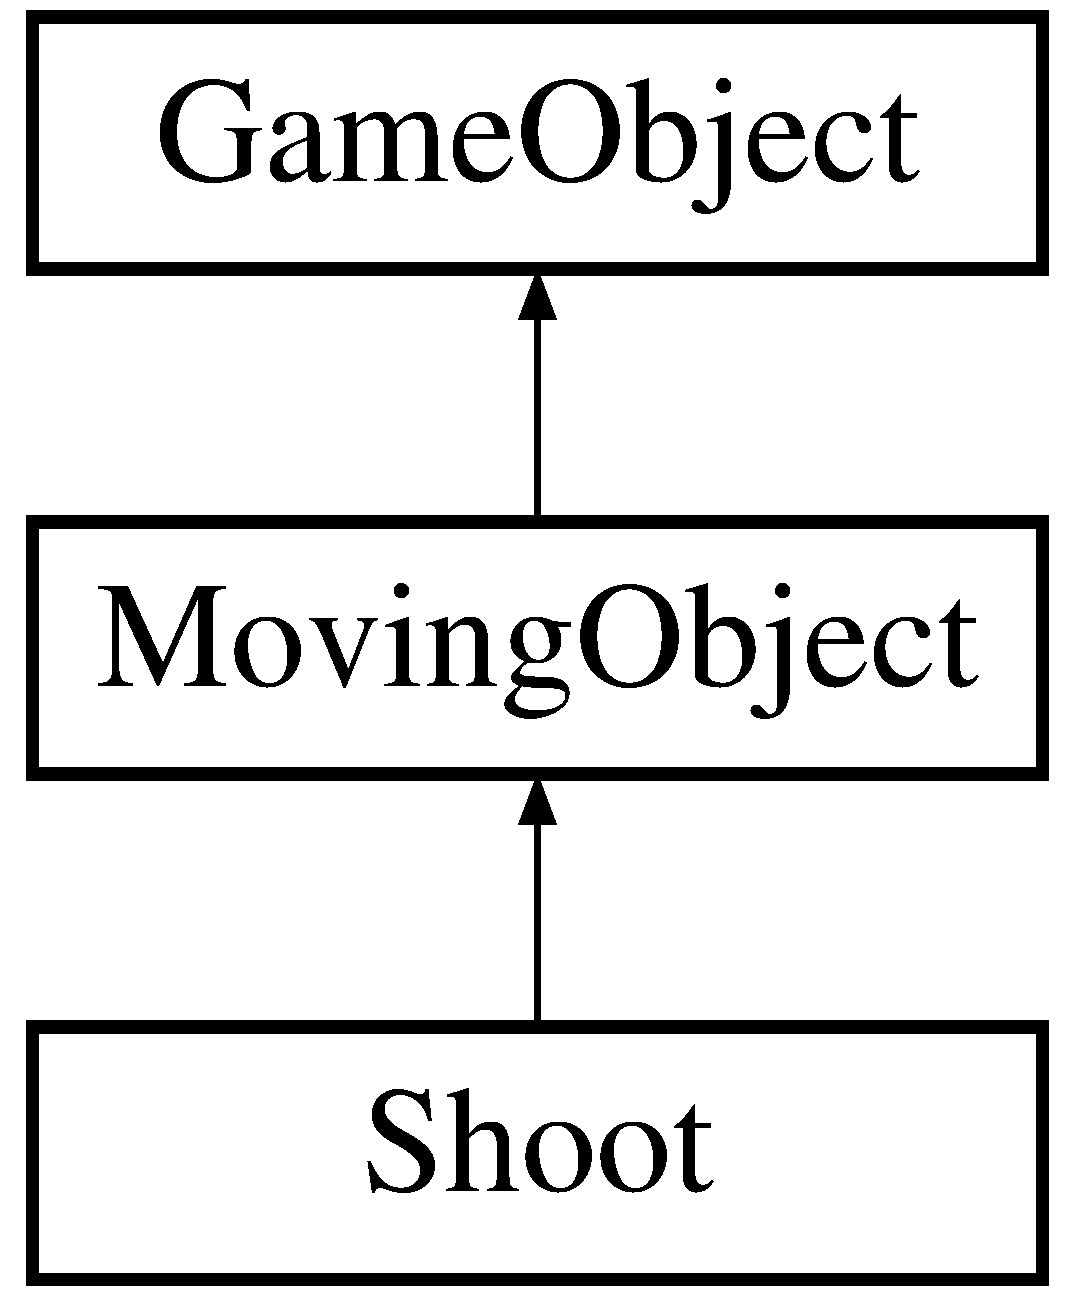
\includegraphics[height=3.000000cm]{classShoot}
\end{center}
\end{figure}
\subsection*{Öffentliche Methoden}
\begin{DoxyCompactItemize}
\item 
\hypertarget{classShoot_a743efe2b8b84053510208ca04ef7638d}{int {\bfseries get\-Inflicted\-Damage} () const }\label{classShoot_a743efe2b8b84053510208ca04ef7638d}

\item 
\hypertarget{classShoot_a9d3509d5698be3d6e7e29f5483d988c7}{void {\bfseries update} ()}\label{classShoot_a9d3509d5698be3d6e7e29f5483d988c7}

\end{DoxyCompactItemize}
\subsection*{Weitere Geerbte Elemente}


Die Dokumentation für diese Klasse wurde erzeugt aufgrund der Dateien\-:\begin{DoxyCompactItemize}
\item 
Wiesn-\/\-Run/src/shoot.\-h\item 
Wiesn-\/\-Run/src/shoot.\-cpp\end{DoxyCompactItemize}

\hypertarget{structstateStruct}{\section{state\-Struct Strukturreferenz}
\label{structstateStruct}\index{state\-Struct@{state\-Struct}}
}


Struktur für die States des Spiels Sowohl Sound-\/ als auch Grafik-\/\-Ausgabe erhalten aus den States Informationen darüber, was gerade im Spiel passiert, z.\-B. dass gerade der Spieler angreift, ein Gegner stribt etc.  




{\ttfamily \#include $<$definitions.\-h$>$}

\subsection*{Öffentliche Attribute}
\begin{DoxyCompactItemize}
\item 
\hypertarget{structstateStruct_a4eae1df10359bedc38b87055681055ec}{bool {\bfseries player\-Jumping}}\label{structstateStruct_a4eae1df10359bedc38b87055681055ec}

\item 
\hypertarget{structstateStruct_ada25e145c4d86fb21994c48730a288fc}{bool {\bfseries player\-Attacking}}\label{structstateStruct_ada25e145c4d86fb21994c48730a288fc}

\item 
\hypertarget{structstateStruct_a66b968e44adb90338ae412b36e72a839}{bool {\bfseries player\-Running}}\label{structstateStruct_a66b968e44adb90338ae412b36e72a839}

\item 
\hypertarget{structstateStruct_adbcc2c3a405e6b6a3f964ddc4fc87fdd}{bool player\-Throwing bool {\bfseries player\-Hit}}\label{structstateStruct_adbcc2c3a405e6b6a3f964ddc4fc87fdd}

\item 
\hypertarget{structstateStruct_a2e86c5f98d0193f81b3724199118d95a}{bool {\bfseries game\-Over}}\label{structstateStruct_a2e86c5f98d0193f81b3724199118d95a}

\item 
\hypertarget{structstateStruct_af6b4e3617286abcbed41129554a762d9}{bool {\bfseries enemy\-Hit}}\label{structstateStruct_af6b4e3617286abcbed41129554a762d9}

\item 
\hypertarget{structstateStruct_a15b4e5c7a787ed565447cc499a5578eb}{bool {\bfseries enemy\-Attacking}}\label{structstateStruct_a15b4e5c7a787ed565447cc499a5578eb}

\item 
\hypertarget{structstateStruct_ac3a06cac79657050c693ff9f2d2ae7ee}{bool {\bfseries enemy\-Throwing}}\label{structstateStruct_ac3a06cac79657050c693ff9f2d2ae7ee}

\item 
\hypertarget{structstateStruct_a4cd54e83a595423b7436198e0bf38f7d}{bool {\bfseries enemy\-Dead}}\label{structstateStruct_a4cd54e83a595423b7436198e0bf38f7d}

\item 
\hypertarget{structstateStruct_a312d8cc1f971d0af0e50e32fa211dabd}{bool {\bfseries beer\-Collected}}\label{structstateStruct_a312d8cc1f971d0af0e50e32fa211dabd}

\item 
\hypertarget{structstateStruct_afa008904c30c42f15869572d67001214}{bool {\bfseries chicken\-Collected}}\label{structstateStruct_afa008904c30c42f15869572d67001214}

\end{DoxyCompactItemize}


\subsection{Ausführliche Beschreibung}
Struktur für die States des Spiels Sowohl Sound-\/ als auch Grafik-\/\-Ausgabe erhalten aus den States Informationen darüber, was gerade im Spiel passiert, z.\-B. dass gerade der Spieler angreift, ein Gegner stribt etc. 

\begin{DoxyRefDesc}{Noch zu erledigen}
\item[\hyperlink{todo__todo000002}{Noch zu erledigen}]Es fehlen noch die States selbst. \begin{DoxyAuthor}{Autor}
Simon 
\end{DoxyAuthor}
\end{DoxyRefDesc}


Die Dokumentation für diese Struktur wurde erzeugt aufgrund der Datei\-:\begin{DoxyCompactItemize}
\item 
Wiesn-\/\-Run/src/definitions.\-h\end{DoxyCompactItemize}

%--- End generated contents ---

% Index
\newpage
\phantomsection
\addcontentsline{toc}{chapter}{Index}
\printindex

\end{document}
